\chapter[Evaluation]{Evaluation}
\label{cp:evaluation}

{
	\parindent0pt
	This chapter presents the scenarios and criteria employed in the evaluation of our implementation. \autoref{sec:benchmark_scenarios} introduces a series of benchmarking scenarios, which have been chosen to reflect distinct simulation characteristics that may appear in real-world applications. Subsequently, \autoref{sec:metrics} defines the evaluation metrics applied to the benchmarks. These metrics are intended to provide comparability between simulation runs with dynamically initiated tuning intervals and to the baseline runs with tuning at fixed frequency.
	Finally, \autoref{sec:default_params} will shortly outline how default values for the newly introduced trigger parameters can be obtained.
}


\section{Benchmarking Scenarios}
\label{sec:benchmark_scenarios}
As to not limit our analysis to one specific simulation setting, we use a selection of benchmarking scenarios that represent different basic particle structures.
The heating-sphere and exploding-liquid scenarios are based on the configuration files given by Newcome et al., adapted and parametrized for use in this thesis \cite{Newcome2025}.
The other scenarios are are taken from the AutoPas \texttt{md-flexible} application\footnote{\href{https://github.com/AutoPas/AutoPas/tree/master/examples/md-flexible/input}{\texttt{https://github.com/AutoPas/AutoPas/tree/master/examples/md-flexible/input}}}.


\pgfplotsset{
	colormap={fast}{
			rgb255(0cm)=(14,14,119);
			rgb255(0.17159223942480895cm)=(61,117,206);
			rgb255(0.2984914818394138cm)=(90,189,243);
			rgb255(0.4321287371255907cm)=(175,237,234);
			rgb255(0.5cm)=(229,240,196);
			rgb255(0.5882260353170073cm)=(244,212,129);
			rgb255(0.7061412605695164cm)=(236,158,80);
			rgb255(0.8476395308725272cm)=(204,89,40);
			rgb255(1cm)=(150,19,30);
		}
}

\newcommand{\fastcolorbar}{%
	\centering
	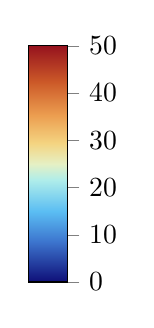
\begin{tikzpicture}
		\pgfplotscolorbardrawstandalone[
			colorbar,
			colormap name=fast,
			point meta min=0,
			point meta max=50,
			colorbar style={
					height=3cm,
					ytick={0,10,...,50},
					tick align=outside,
					tick pos=right,
				},
		]
	\end{tikzpicture}

	\begin{tikzpicture}
		\node[anchor=north, align=center] at (0,0) {\si{F^{*}}};
	\end{tikzpicture}
}

\newcommand{\fastcolorbarhor}{%
	\centering
	\begin{tikzpicture}
		\node[anchor=east, align=center] at (-0.25cm,-0.25cm) {\si{F^{*}}};
		\pgfplotscolorbardrawstandalone[
			colorbar horizontal,
			colormap name=fast,
			point meta min=0,
			point meta max=50,
			colorbar style={
					width=3cm,
					xtick={0,10,...,50},
					tick align=outside,
					tick pos=top,
					xticklabel pos=top,
				},
		]
	\end{tikzpicture}
}


\subsection{Equilibrium}
\label{subsec:scenario_equil}
In the equilibrium scenario (\autoref{fig:evolution_equil}), particles are packed tightly into a cube, with periodic boundary conditions imposed on the simulation space. Periodic boundary conditions ensure that particles exiting the simulation domain on one side are reinserted on the opposite side. First, the particles interactions with each other loosens up the grid structure, but ultimately an equilibrium is reached in which no significant changes in particle positions occur anymore. After that initial relaxation, no further scenario change expected. Therefore, no additional tuning phases should be needed in the equilibrium phase, as the optimal configuration is not expected to change.

\begin{figure}[htpb]
	\centering
	\begin{subfigure}[c]{.3\textwidth}
		\includegraphics[width=\textwidth]{equilibrium/render/t0.png}
		\subcaption{Iteration \num{0}} % 0, 0
	\end{subfigure}%
	\begin{subfigure}[c]{.3\textwidth}
		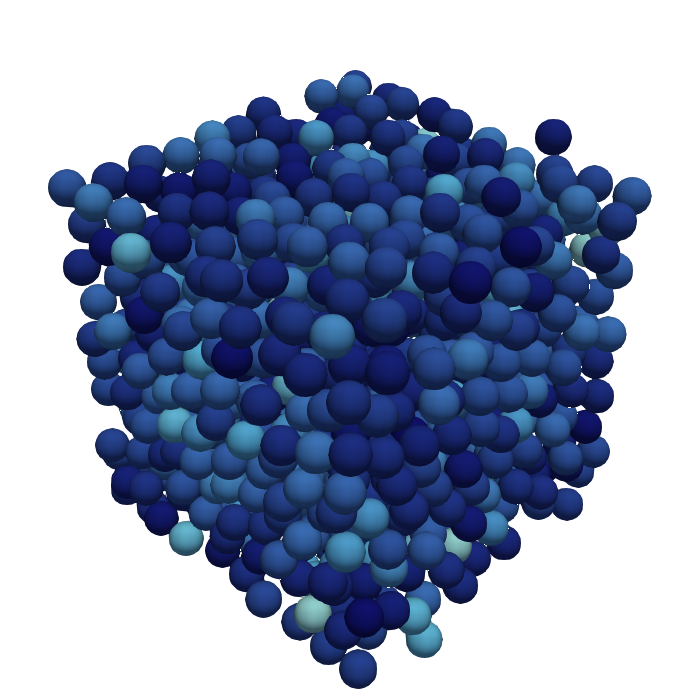
\includegraphics[width=\textwidth]{equilibrium/render/t10000.png}
		\subcaption{Iteration \num{10000}} % 10000, 10
	\end{subfigure}%
	\begin{subfigure}[c]{.3\textwidth}
		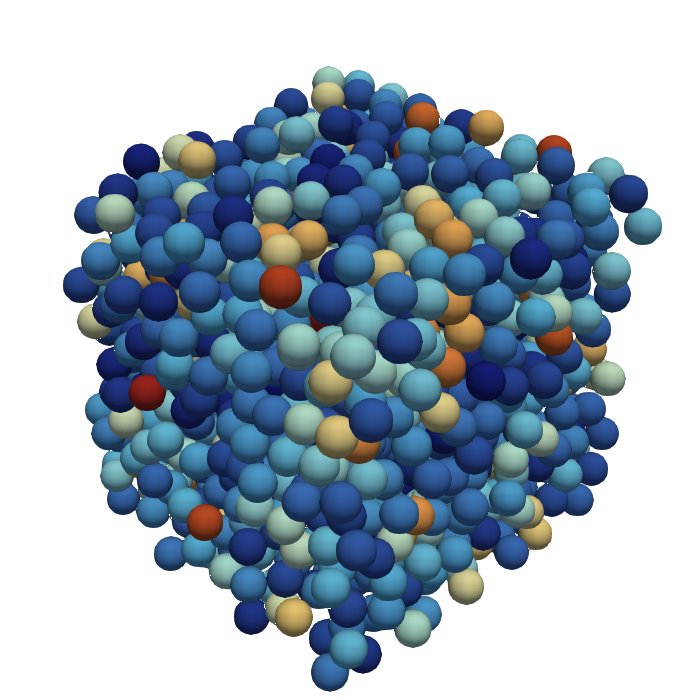
\includegraphics[width=\textwidth]{equilibrium/render/t50000.png}
		\subcaption{Iteration \num{50000}} % 50000, 50
	\end{subfigure}%
	\hfill\begin{subfigure}[c]{.08\textwidth}
		\fastcolorbar
	\end{subfigure}
	\caption{Evolution of the simulation state in the equilibrium scenario. The coloring indicates the forces acting upon a particle, and is given in reduced units. Note that the overall forces decrease as the equilibrium is reached, even tough the specific timestamps depicted might suggest otherwise.}
	\label{fig:evolution_equil}
\end{figure}


\subsection{Exploding Liquid}
\label{subsec:scenario_expl}
Similarly to the equilibrium scenario, the exploding-liquid scenario (\autoref{fig:evolution_expl}) starts off with the particles packed into a cuboid, with periodic boundaries imposed on the simulation space. The cuboid explodes in $y$-direction and collides with the boundary. This leads to multiple waves of particles with decreasing intensity, until the simulation finally settles into an equilibrium state, with particles spread out over the whole domain. If a single autotuning instance is used for the whole domain, the rapid changes in particle positions and heterogeneous particle distribution make finding an optimal configuration very hard. However, if the domain is split up into multiple independent AutoPas instances on different MPI nodes, each autotuning instance can independently find an optimal configuration for its part of the domain. Using this, the simulation domain can be split up into regions with high particle density and velocities and regions with little to no particles.

\begin{figure}[htpb]
	\centering
	\begin{subfigure}[c]{.25\textwidth}
		\newsavebox{\colorbarbox}
		\savebox{\colorbarbox}{
			\fastcolorbarhor
		}
		\usebox{\colorbarbox}%
		\vspace*{-\ht\colorbarbox} %
		\includegraphics[width=\textwidth]{exploding-liquid/render/t0.png}
		\subcaption{Iteration \num{0}} % 0 
	\end{subfigure}%
	\begin{subfigure}[c]{.25\textwidth}
		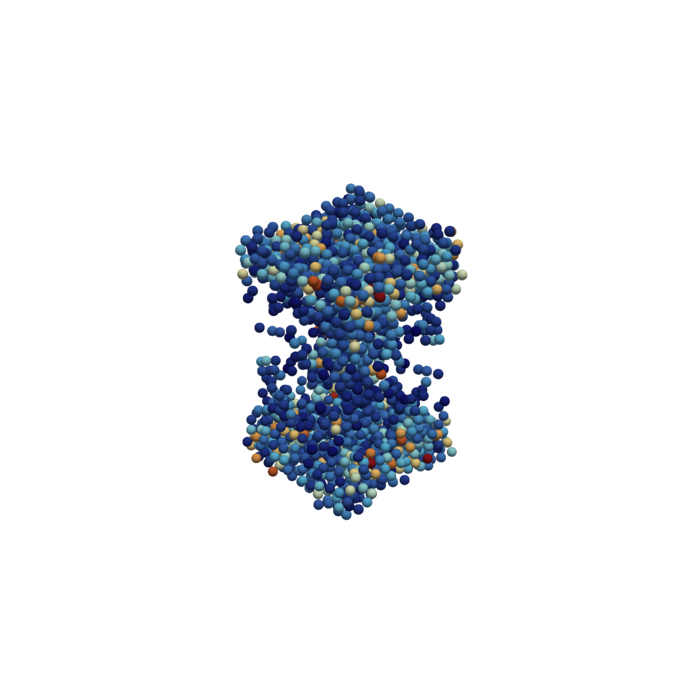
\includegraphics[width=\textwidth]{exploding-liquid/render/t3000.png}
		\subcaption{Iteration \num{3000}} % 3000, 5.5
	\end{subfigure}%
	\begin{subfigure}[c]{.25\textwidth}
		\centering
		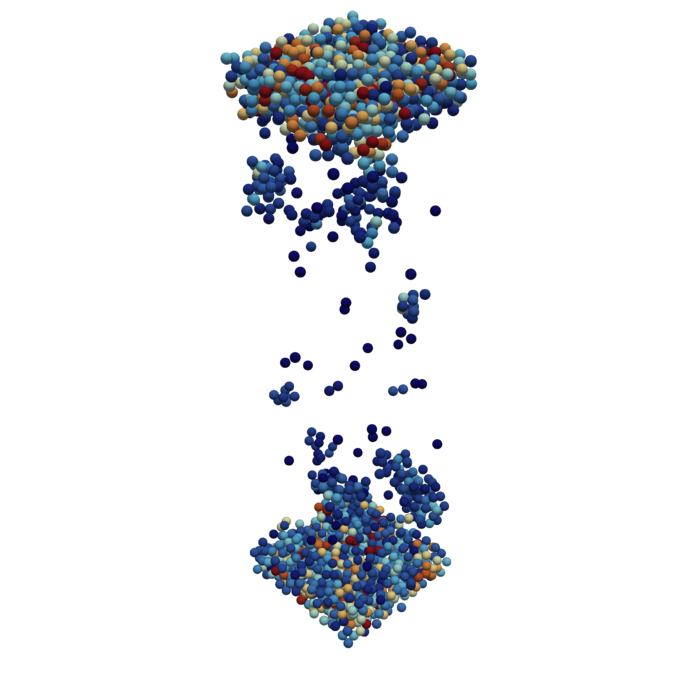
\includegraphics[width=\textwidth]{exploding-liquid/render/t11000.png}
		\subcaption{Iteration \num{11000}} % 11000, 20
	\end{subfigure}%
	\begin{subfigure}[c]{.25\textwidth}
		\centering
		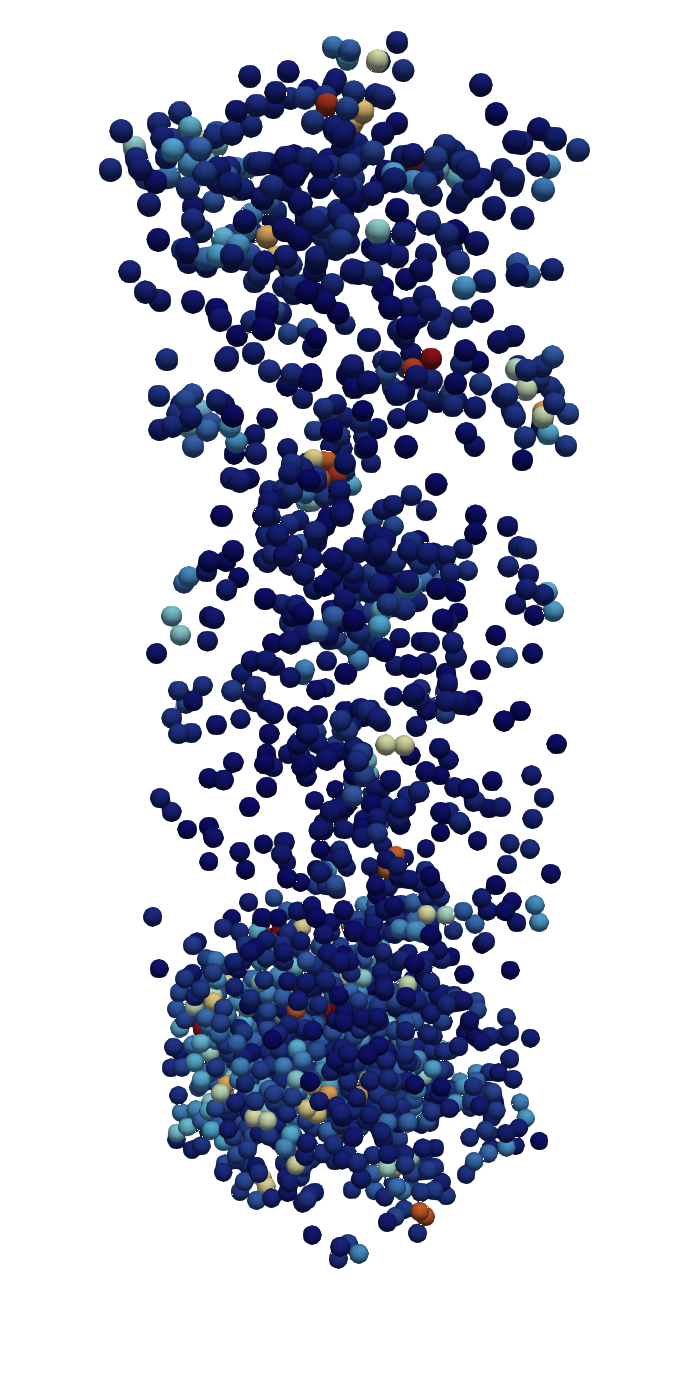
\includegraphics[width=\textwidth]{exploding-liquid/render/t31000.png}
		\subcaption{Iteration \num{31000}} % 31000, ?? 
	\end{subfigure}
	\caption{Evolution of the simulation state in the exploding-liquid scenario.}
	\label{fig:evolution_expl}
\end{figure}

\subsection{Heating Sphere}
\label{subsec:scenario_hs}
The heating-sphere scenario (\autoref{fig:evolution_hs}) starts off with a dense, small sphere of particles. In contrast to the previously introduced scenarios, reflective boundary conditions are applied. Over the course of the simulation, the temperature rises from \num{0.1} to \num{100} with a change of $\Delta \si{T^{*}}=0.1$ every \num{100} iterations. Additionally, Brownian motion is applied, i.e., random fluctuations in particle positions \cite{Moerters2010}. The sphere expands with the increasing temperature and particles slowly radiate outwards. In the late phase of the simulation, particles are spread out across the whole domain.
Between the initial, compacted state and the equilibrated state, the optimal configuration changes.

\begin{figure}[htpb]
	\centering
	\fastcolorbarhor
	\vspace*{\baselineskip}
	\begin{subfigure}{.25\textwidth}
		\includegraphics[draft=false,width=\textwidth]{heating-sphere/render/t0.png}
		\subcaption{Iteration \num{0}} % 0
	\end{subfigure}%
	\begin{subfigure}{.25\textwidth}
		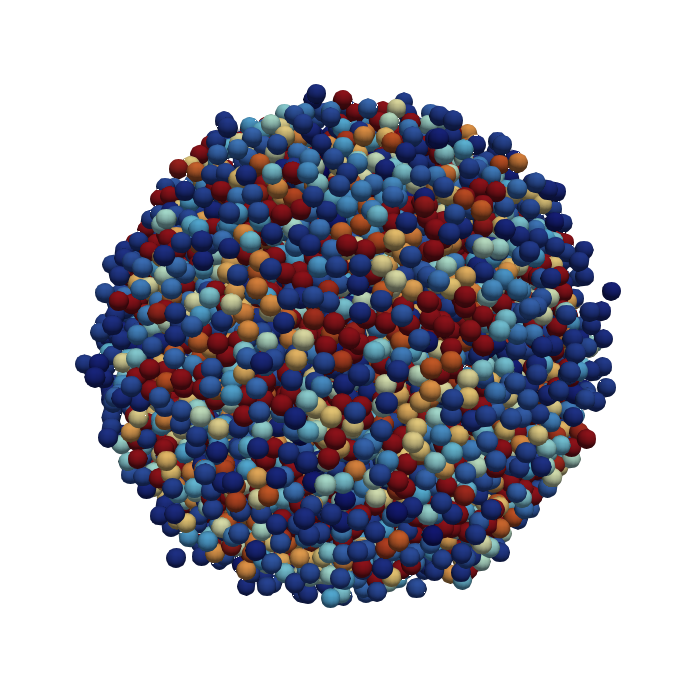
\includegraphics[draft=false,width=\textwidth]{heating-sphere/render/t4000.png}
		\subcaption{Iteration \num{4000}} % 4000, 0.4
	\end{subfigure}%
	\begin{subfigure}{.25\textwidth}
		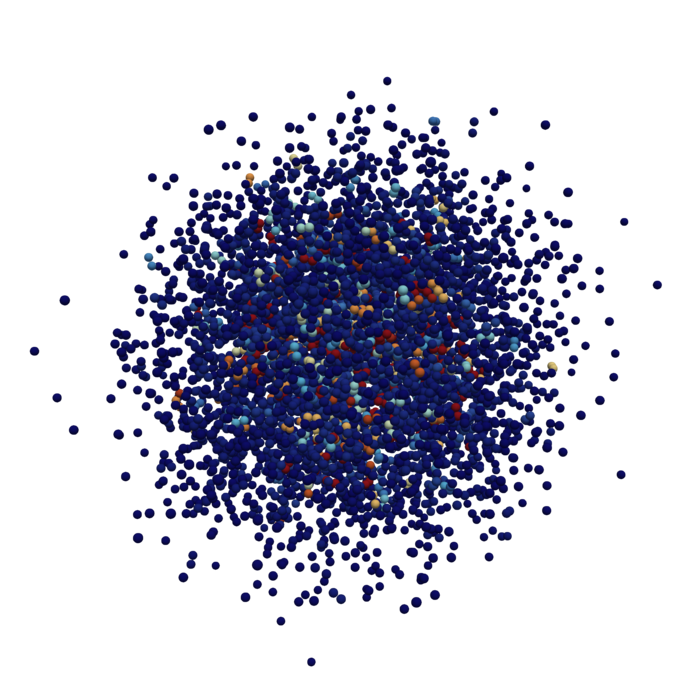
\includegraphics[draft=false,width=\textwidth]{heating-sphere/render/t23000.png}
		\subcaption{Iteration \num{23000}} % 23000, 2.3
	\end{subfigure}%
	\begin{subfigure}{.25\textwidth}
		\vspace*{0.1\textwidth}
		\centering
		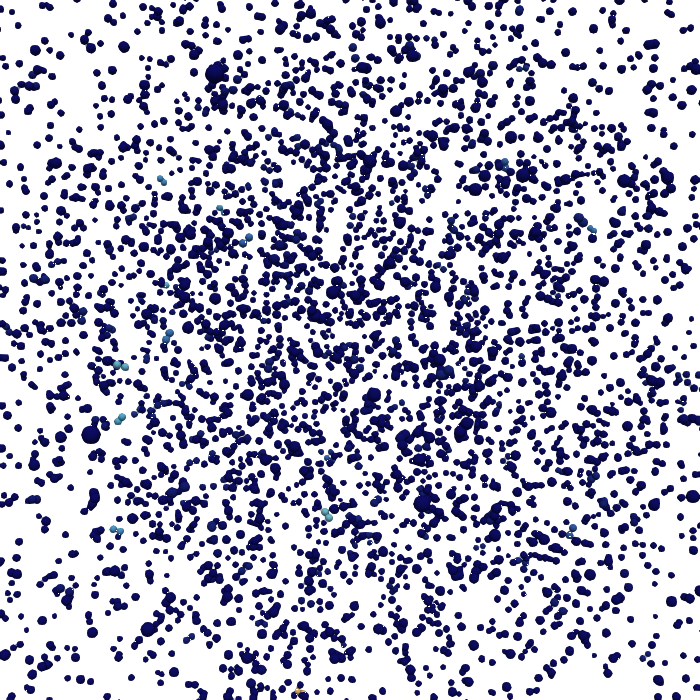
\includegraphics[width=0.8\textwidth]{heating-sphere/render/t60000.png}
		\vspace*{0.1\textwidth}
		\subcaption{Iteration \num{60000}} % 60000, 6
	\end{subfigure}%
	\caption{Evolution of the simulation state in the heating-sphere scenario.}
	\label{fig:evolution_hs}
\end{figure}

%\subsection{Falling Drop}
%\label{subsec:fd}
%\subsection{Spinodial Decomposition}
%\label{subsec:sd}

\section{Evaluation Metrics}
\label{sec:metrics}
To compare results between our dynamic initiation of tuning phases and the currently implemented static approach, we use multiple metrics.
The primary goal is to reduce the total simulation runtime for a range of typical scenarios; it is therefore our first metric. As tuning phases spend time in quite suboptimal configurations, a reduction in total runtime is the expected result if our approach reduces the number of tuning phases without computing too many iterations using a suboptimal configuration.

The metric of total runtime is not particularly fine-grained, however, as it only takes into account entire simulation runs. To achieve a more detailed benchmark, we also consider the number of iterations that were computed using the optimal configuration. As an approximate baseline, we use simulation runs with short, fixed tuning intervals. Based on this approximation we can then rank the configuration our implementation chose in terms of optimality.

Finally, we also consider the number of tuning phases initiated or, more precisely, the number of tuning iterations over the course of the whole simulation. Otherwise, we could not differentiate whether any achieved speedup is due to our trigger strategies or the fact that not triggering any tuning phases at all was more efficient for a given scenario.

\section{Default Trigger Parameters}
\label{sec:default_params}
All presented trigger strategies are based on a user-set trigger factor $\lambda$. The averaging, split and regression triggers additionally take into account the number of samples to inspect, denoted as $n$. For any dynamic tuning trigger to be useful, reasonable default values for these parameters are needed, as the performance of the whole simulation is dependent on the trigger's behavior.
Furthermore, optimal values for these parameters may depend on the scenario, trigger strategy or both.
Reasonable default values can be found by comparing a range of combinations $\left(\lambda_i, n_j\right)$ for any given scenario and trigger strategy.



